%% chapter2_slides.tex
%% Beamer slides for Chapter 2: Notation and Mathematical Foundations
%% "The Krasnosel'skii-Mann Iterative Method: Recent Progress and Applications"
%% Dong, Cho, He, Pardalos & Rassias -- SpringerBriefs in Optimization, 2022
%% Reader-friendly style: complete sentences, symbol explanations, worked examples
%% Compiled with: pdflatex -interaction=nonstopmode chapter2_slides.tex  (twice)
\documentclass[aspectratio=169,10pt]{beamer}

\usetheme{Madrid}
\usecolortheme{seahorse}
\usefonttheme{professionalfonts}

%% ── Packages ──────────────────────────────────────────────────────────────
\usepackage{amsmath,amssymb,amsfonts}
\usepackage{mathtools}
\usepackage{graphicx}
\usepackage{booktabs}
\usepackage{xcolor}
\usepackage{listings}

\graphicspath{{figures/}}

%% ── Python listing style ─────────────────────────────────────────────────
\lstdefinestyle{pycode}{
  language=Python,
  basicstyle=\ttfamily\scriptsize,
  numbers=left,
  numberstyle=\tiny\color{gray},
  frame=single,
  backgroundcolor=\color{gray!7},
  keywordstyle=\color{blue!70!black}\bfseries,
  commentstyle=\color{green!50!black}\itshape,
  stringstyle=\color{orange!80!black},
  showstringspaces=false,
  breaklines=true,
  tabsize=4,
  xleftmargin=1.5em,
  framexleftmargin=1.5em,
  aboveskip=4pt,
  belowskip=4pt,
}

%% ── Metadata ─────────────────────────────────────────────────────────────
\title[KM Method -- Ch.2]{The Krasnosel'ski\u{i}-Mann Iterative Method}
\subtitle{Chapter 2: Notation and Mathematical Foundations}
\author{Based on Dong, Cho, He, Pardalos \& Rassias}
\date{SpringerBriefs in Optimization, 2022}

\setbeamertemplate{footline}[frame number]
\setbeamertemplate{navigation symbols}{}

%% ── Helper macros ─────────────────────────────────────────────────────────
\DeclareMathOperator{\Fix}{Fix}
\DeclareMathOperator{\dom}{dom}
\DeclareMathOperator{\ran}{ran}
\DeclareMathOperator{\gra}{gra}
\DeclareMathOperator{\zer}{zer}
\DeclareMathOperator*{\argmin}{argmin}
\newcommand{\Id}{\mathrm{Id}}
\newcommand{\R}{\mathbb{R}}
\newcommand{\wto}{\rightharpoonup}

%% ══════════════════════════════════════════════════════════════════════════
\begin{document}

%% ── Title frame ──────────────────────────────────────────────────────────
\begin{frame}
  \titlepage
\end{frame}

%% ── Outline ──────────────────────────────────────────────────────────────
\begin{frame}{Chapter Overview}
  \tableofcontents
\end{frame}

\AtBeginSection[]{\begin{frame}{Outline}\tableofcontents[currentsection]\end{frame}}

%% ══════════════════════════════════════════════════════════════════════════
\section{Overview and the Running Example}
%% ══════════════════════════════════════════════════════════════════════════

\begin{frame}[allowframebreaks]{Why This Chapter Matters}

Every later chapter in this book studies iterative algorithms of the form
$x_{n+1} = T(x_n)$ or blends of such maps, and every convergence proof leans on
a small, fixed vocabulary of operator properties (nonexpansive, averaged,
monotone, \ldots) and a handful of standard inequalities. This chapter
\emph{is} that vocabulary. Nothing here is specific to the
Krasnosel'ski\u{i}--Mann (KM) method yet --- instead we build the toolbox that
every subsequent chapter's proofs will reach into without re-explaining.

  \begin{block}{How to Read This Chapter}
    We will introduce each definition in plain English with an analogy first,
    then give the exact formula from the book, then check the definition
    against a single concrete, running numerical example so that the abstract
    symbols always have a ``home'' you can compute by hand.
  \end{block}

  \begin{alertblock}{The Running Example (used throughout this deck)}
    Let $\mathcal{H} = \R^2$ with the usual dot product, and let
    \[
      C = \{\, z \in \R^2 : \|z\| \le 1 \,\}
    \]
    be the \textbf{closed unit disk}. Let $P_C : \R^2 \to C$ be the
    \textbf{metric projection} onto $C$ (formally defined later in this
    chapter): $P_C(x)$ is the point of $C$ closest to $x$. For $x$ outside the
    disk this is $P_C(x) = x/\|x\|$ (rescale $x$ down to the unit circle); for
    $x$ already inside $C$, $P_C(x) = x$. We will repeatedly use the two
    points
    \[
      x = (3, 4), \qquad y = (0, 2).
    \]
    Since $\|x\| = 5 > 1$, $P_C(x) = x/5 = (0.6,\, 0.8)$.
    Since $\|y\| = 2 > 1$, $P_C(y) = y/2 = (0,\, 1)$.
    Every operator class introduced below will be checked against this pair.
  \end{alertblock}

\end{frame}

%% ══════════════════════════════════════════════════════════════════════════
\section{Part (A): Notation}
%% ══════════════════════════════════════════════════════════════════════════

\begin{frame}[allowframebreaks]{Notation You'll Need: Basic Objects}

  \begin{block}{Spaces and the Ambient Setting}
    Throughout the book, $\mathbb{N}$ denotes the set of nonnegative
    integers, and $\mathcal{H}$ and $\mathcal{G}$ denote real
    \textbf{Hilbert spaces} with inner product $\langle \cdot, \cdot \rangle$
    and norm $\|\cdot\|$. A Hilbert space is simply a vector space equipped
    with a notion of angle/inner product $\langle a, b\rangle$ (from which the
    length $\|a\| = \sqrt{\langle a, a\rangle}$ and the distance
    $\|a-b\|$ are built) that is ``complete'' (no missing limit points). If
    you have never seen the general definition, it is safe to think of
    $\mathcal{H}$ as a (possibly infinite-dimensional) generalization of
    $\R^N$, the standard $N$-dimensional Euclidean space, which is itself
    always a valid (finite-dimensional) Hilbert space. \textbf{Every concrete
    example and Python computation in this deck lives in $\mathcal{H} = \R^2$},
    the plane, so you can always picture points as arrows from the origin.
  \end{block}

  \begin{block}{Weak Convergence $\wto$ versus Strong Convergence $\to$}
    We write $x_n \to x$ for \textbf{strong (ordinary) convergence}: the
    distance $\|x_n - x\| \to 0$ as $n \to \infty$. We write $x_n \wto x$ for
    \textbf{weak convergence}: $\langle x_n, v \rangle \to \langle x, v
    \rangle$ for \emph{every fixed} $v \in \mathcal{H}$, even though the
    points $x_n$ themselves need not get uniformly close to $x$ in distance.

    \medskip
    \textbf{Intuition.} Strong convergence says ``the points really do get
    close, measured directly.'' Weak convergence only says ``every fixed
    measurement (projection onto a direction $v$) of $x_n$ eventually agrees
    with the same measurement of $x$.'' In finite dimensions ($\R^N$, which is
    where every example in this deck lives), \textbf{these two notions
    coincide exactly}: $x_n \to x$ if and only if $x_n \wto x$. So in $\R^2$
    you may freely read $\wto$ as ``$\to$.''
  \end{block}

  \framebreak

  \begin{alertblock}{Why the Distinction Matters at All (a Flag for Later)}
    In \emph{infinite}-dimensional Hilbert spaces, weak and strong convergence
    genuinely differ, and several later chapters' convergence proofs only
    obtain the \emph{weaker} conclusion $x_n \wto x^*$. The classic example:
    let $(e_n)_{n \in \mathbb{N}}$ be an orthonormal sequence in
    $\ell^2$ (e.g., $e_n$ has a $1$ in coordinate $n$ and $0$ elsewhere). Then
    $e_n \wto 0$ (because $\langle e_n, v \rangle \to 0$ for every fixed
    $v \in \ell^2$, by Bessel's inequality), yet $\|e_n - 0\| = 1$ for
    \emph{every} $n$ --- the sequence never gets close to $0$ in norm, so it
    does \emph{not} converge strongly. Keep this one-sentence example in your
    back pocket: it is the standing reason later chapters must work harder to
    upgrade weak convergence results to strong ones.
  \end{alertblock}

  \begin{block}{The Weak $\omega$-Limit Set $\omega_w(x_n)$}
    For a sequence $\{x_n\}_{n \in \mathbb{N}}$, define
    \[
      \omega_w(x_n) = \{\, x : \exists\, x_{n_j} \wto x \,\}.
    \]
    In words: $\omega_w(x_n)$ collects \emph{every} point that is the weak
    limit of \emph{some} subsequence of $\{x_n\}$ --- the set of all
    ``weak cluster points.'' \textbf{Intuition:} if the whole sequence
    weakly converges to a single point $x$, then $\omega_w(x_n) = \{x\}$
    is a singleton. If the sequence oscillates between two weak limits (like
    $(-1)^n$ oscillating between $-1$ and $1$), $\omega_w(x_n)$ contains both.
    A recurring proof strategy in this book is: show every element of
    $\omega_w(x_n)$ lies in some target set $S$, and separately show
    $\lim_n \|x_n - s\|$ exists for every $s \in S$; together these force
    $x_n \wto$ a single point of $S$ (this is Lemma~2.7 below).
  \end{block}

  \framebreak

  \begin{block}{A Few More Notational Conventions}
    \begin{itemize}
      \item $\ell^1_+$ denotes the set of \textbf{summable sequences} in
        $[0, +\infty)$: nonnegative real sequences $\{a_n\}$ with
        $\sum_{n=0}^{\infty} a_n < +\infty$. These show up as error terms in
        convergence proofs (``as long as the accumulated error is
        summable, it cannot prevent convergence'').
      \item For $\xi \in \R$, the \textbf{positive part} is
        $\xi^+ = \max\{0, \xi\}$ and the \textbf{negative part} is
        $\xi^- = -\min\{0, \xi\}$. Both are always $\ge 0$, and
        $\xi = \xi^+ - \xi^-$ while $|\xi| = \xi^+ + \xi^-$. Think of
        $\xi^+$ as ``the amount by which $\xi$ exceeds $0$'' and $\xi^-$ as
        ``the amount by which $\xi$ falls short of $0$.''
    \end{itemize}
  \end{block}

\end{frame}

\begin{frame}[fragile]{Python: Weak = Strong Convergence in $\R^N$, and $\omega_w(x_n)$}

In finite dimensions, checking weak convergence reduces to checking
$\langle x_n - x, v\rangle \to 0$ for a spanning set of test directions $v$,
equivalent to ordinary convergence $\|x_n - x\| \to 0$. The code verifies
this equivalence, and separately illustrates $\omega_w(x_n)$ for an
oscillating sequence with two cluster points.

\begin{lstlisting}[style=pycode]
import numpy as np
rng = np.random.default_rng(0)

# Part 1: weak convergence == strong convergence in R^2
x_star = np.array([1.0, -2.0])
xs = [x_star + np.array([1.0, 1.0]) / (n + 1) for n in range(1, 2000)]
test_dirs = rng.normal(size=(5, 2))            # 5 fixed test directions v
strong_err = [np.linalg.norm(xn - x_star) for xn in xs]
weak_err = [max(abs(np.dot(xn - x_star, v)) for v in test_dirs) for xn in xs]
print("strong error -> 0? ", strong_err[-1] < 1e-3)
print("weak error   -> 0? ", weak_err[-1] < 1e-3)   # both vanish together

# Part 2: omega_w(x_n) for an oscillating sequence (two cluster points)
a, b = np.array([1.0, 0.0]), np.array([0.0, 1.0])
seq = [a if n % 2 == 0 else b for n in range(20)]
cluster_points = {tuple(a), tuple(b)}
print("omega_w(x_n) =", cluster_points)        # {(1,0), (0,1)}
\end{lstlisting}

\end{frame}

%% ══════════════════════════════════════════════════════════════════════════
\section{Part (B): Classes of Operators}
%% ══════════════════════════════════════════════════════════════════════════

\begin{frame}[allowframebreaks]{Notation You'll Need: Lipschitz, Nonexpansive, Contractive}

  \begin{block}{Definition 2.1 (Lipschitz-Type Operators)}
    An operator $T : \mathcal{H} \to \mathcal{H}$ is said to be:
    \begin{enumerate}
      \item[(1)] \textbf{$L$-Lipschitz continuous} for $L \ge 0$ if
        \[
          \|T(x) - T(y)\| \le L\|x - y\| \quad \text{for all } x, y \in \mathcal{H}.
        \]
      \item[(2)] \textbf{nonexpansive} if $L = 1$.
      \item[(3)] \textbf{contractive} if $0 < L < 1$.
    \end{enumerate}
  \end{block}

  \begin{block}{Plain-English Intuition}
    Lipschitz continuity with constant $L$ says: ``$T$ can stretch distances
    by at most a factor of $L$.'' \textbf{Nonexpansive} ($L=1$) means $T$
    \emph{never stretches distances at all} --- two points can only get
    closer together or stay the same distance apart after applying $T$, never
    farther apart. \textbf{Contractive} ($L<1$) is stronger still: $T$ must
    \emph{strictly shrink} every pair of distances by a fixed factor, which is
    exactly the hypothesis of the Banach fixed-point theorem.
  \end{block}

  \framebreak

  \begin{exampleblock}{Running Example: $P_C$ is Nonexpansive}
    Using $x = (3,4)$, $y=(0,2)$ from before, with $P_C(x) = (0.6, 0.8)$ and
    $P_C(y) = (0, 1)$:
    \[
      \|P_C(x) - P_C(y)\| = \|(0.6,\,-0.2)\| = \sqrt{0.36 + 0.04} = \sqrt{0.4}
        \approx 0.632,
    \]
    \[
      \|x - y\| = \|(3, 2)\| = \sqrt{9+4} = \sqrt{13} \approx 3.606.
    \]
    Indeed $0.632 \le 3.606$: projecting onto $C$ did not increase the
    distance between the two points. (We verify this holds for \emph{every}
    pair $x,y$, not just this one, in Lemma~2.4 below.)
  \end{exampleblock}

  \begin{block}{Definition 2.2 (Pseudocontractive Operators)}
    An operator $T : \mathcal{H} \to \mathcal{H}$ is \textbf{pseudocontractive}
    if
    \[
      \|T(x) - T(y)\|^2 \le \|x-y\|^2 + \|(\Id - T)x - (\Id-T)y\|^2
      \quad \text{for all } x, y \in \mathcal{H}.
    \]
    Here $\Id$ is the \textbf{identity operator}, $\Id(x) = x$. The class of
    pseudocontractive operators \emph{includes} the nonexpansive operators:
    if $T$ is nonexpansive, the extra term
    $\|(\Id-T)x - (\Id-T)y\|^2 \ge 0$ only makes the right-hand side larger,
    so the inequality $\|T(x)-T(y)\|^2 \le \|x-y\|^2 \le \|x-y\|^2 +
    \|(\Id-T)x-(\Id-T)y\|^2$ holds automatically. Pseudocontractive operators
    are thus a strictly larger, more permissive class.
  \end{block}

\end{frame}

\begin{frame}[allowframebreaks]{Notation You'll Need: Demicontractive and Quasi-nonexpansive Operators}

  \begin{block}{Definition 2.3 ($k$-Demicontractive Operators)}
    An operator $T : \mathcal{H} \to \mathcal{H}$ \textbf{with a fixed point}
    (recall $\Fix(T) = \{x \in \mathcal{H} : T(x) = x\}$, the set of points
    left unchanged by $T$) is said to be:
    \begin{enumerate}
      \item[(1)] \textbf{$k$-demicontractive} for $k \in \R$ if
        \[
          \|T(x) - y\|^2 \le \|x-y\|^2 + k\|T(x) - x\|^2
          \quad \text{for all } x \in \mathcal{H}, \; y \in \Fix(T).
        \]
      \item[(2)] \textbf{quasi-nonexpansive} if $k = 0$, i.e.
        $\|T(x) - y\| \le \|x - y\|$ for all $x \in \mathcal{H}$,
        $y \in \Fix(T)$.
    \end{enumerate}
  \end{block}

  \begin{block}{Plain-English Intuition}
    These definitions only constrain how $T$ behaves \emph{relative to its
    own fixed points} $y \in \Fix(T)$, not relative to arbitrary pairs of
    points. Quasi-nonexpansive says: ``every point moves strictly closer to
    (or no farther from) every fixed point after applying $T$.'' This is
    weaker than nonexpansiveness, which demands the distance-preserving
    property for \emph{all} pairs $x,y \in \mathcal{H}$, fixed points or not.
    \textbf{If $T$ has a fixed point and is nonexpansive, then $T$ is
    automatically quasi-nonexpansive} (just specialize $y$ to be a fixed
    point in the nonexpansive inequality), \textbf{but the reverse is not
    necessarily true} --- there are quasi-nonexpansive maps that stretch
    distances between two arbitrary (non-fixed) points.
  \end{block}

  \framebreak

  \begin{exampleblock}{Running Example: $P_C$ is Quasi-nonexpansive}
    $\Fix(P_C) = C$ itself: every point already in the unit disk is left
    unchanged, and no point outside $C$ is fixed. Since $P_C$ is nonexpansive
    (previous frame) and has fixed points, it is automatically
    quasi-nonexpansive: for any $x \in \R^2$ and any $y \in C$,
    $\|P_C(x) - y\| \le \|x - y\|$. Take $x = (3,4)$ and the fixed point
    $y = (0.6, 0.8) \in C$ (an arbitrary boundary point of $C$):
    \[
      \|P_C(x) - y\| = \|(0.6,0.8)-(0.6,0.8)\| = 0 \le \|x - y\| = \|(2.4, 3.2)\| = 4.
    \]
  \end{exampleblock}

\end{frame}

\begin{frame}[allowframebreaks]{Firmly Nonexpansive Operators}

  \begin{block}{Definition 2.4 (Firmly Nonexpansive)}
    An operator $T : \mathcal{H} \to \mathcal{H}$ is said to be
    \textbf{firmly nonexpansive} if
    \[
      \|T(x) - T(y)\|^2 \le \langle T(x) - T(y),\, x - y \rangle
      \quad \text{for all } x, y \in \mathcal{H}.
    \]
  \end{block}

  \begin{block}{Plain-English Intuition}
    Firm nonexpansiveness is a \emph{stronger}, better-behaved kind of
    nonexpansiveness. Geometrically, it says the vector $T(x)-T(y)$ and the
    vector $x-y$ point in a sufficiently ``aligned'' direction that their
    inner product dominates the squared length of $T(x)-T(y)$ --- think of
    it as ``the image points can never overshoot, and in fact the angle
    between the displacement of the inputs and the displacement of the
    outputs is never obtuse.'' \textbf{If $T$ is firmly nonexpansive, then
    $T$ is nonexpansive}: by the Cauchy--Schwarz inequality,
    \[
      \|T(x)-T(y)\|^2 \le \langle T(x)-T(y), x-y\rangle
      \le \|T(x)-T(y)\|\,\|x-y\|,
    \]
    and dividing both sides by $\|T(x)-T(y)\|$ (when nonzero) gives
    $\|T(x)-T(y)\| \le \|x-y\|$.
  \end{block}

  \framebreak

  \begin{block}{Lemma 2.1 (Equivalent Characterization)}
    Let $T : \mathcal{H} \to \mathcal{H}$. The following are equivalent:
    \begin{enumerate}
      \item[(1)] $T$ is firmly nonexpansive.
      \item[(2)] $2T - \Id$ is nonexpansive.
    \end{enumerate}
  \end{block}

  \begin{block}{Step-by-Step Verification for $P_C$ (Lemma 2.4(1))}
    We verify that $P_C$ is firmly nonexpansive using the running example
    $x=(3,4)$, $y=(0,2)$, $P_C(x)=(0.6,0.8)$, $P_C(y)=(0,1)$:
    \[
      \text{LHS} = \|P_C(x)-P_C(y)\|^2 = \|(0.6,-0.2)\|^2 = 0.36+0.04 = 0.4,
    \]
    \[
      \text{RHS} = \langle P_C(x)-P_C(y),\, x-y\rangle
       = \langle (0.6,-0.2), (3,2)\rangle = 1.8 - 0.4 = 1.4.
    \]
    Indeed $0.4 \le 1.4$, confirming the firmly-nonexpansive inequality for
    this pair. (Below we derive this fact for \emph{all} $x,y$, using the
    variational characterization of the projection.)
  \end{block}

  \framebreak

  \begin{block}{Definition 2.5 ($\alpha$-Averaged Operators)}
    Let $T : \mathcal{H} \to \mathcal{H}$. For $\alpha \in (0,1)$, $T$ is said
    to be \textbf{$\alpha$-averaged} if there exists a nonexpansive operator
    $S : \mathcal{H} \to \mathcal{H}$ such that
    \[
      T = \alpha S + (1-\alpha)\Id.
    \]
  \end{block}

  \begin{block}{Plain-English Intuition}
    An averaged operator is a \textbf{weighted blend of the identity map and a
    nonexpansive map}: applying $T$ means moving only a fraction $\alpha$ of
    the way from ``do nothing'' ($\Id$) toward ``apply the nonexpansive map
    $S$.'' This ``partial step'' structure is \emph{literally what powers the
    Krasnosel'ski\u{i}--Mann iteration}: $x_{n+1} = (1-\alpha_n)x_n +
    \alpha_n T(x_n)$ is precisely an averaging step, and understanding when
    the resulting map is averaged (hence well-behaved) is central to the rest
    of this book.
  \end{block}

  \begin{block}{Remark 2.1}
    If $T$ is firmly nonexpansive, then $T$ is $\tfrac{1}{2}$-averaged.
    (Proof: by Lemma~2.1, $S := 2T - \Id$ is nonexpansive, and rearranging
    gives exactly $T = \tfrac{1}{2}S + \tfrac{1}{2}\Id$.)
  \end{block}

  \framebreak

  \begin{exampleblock}{Running Example: $P_C$ Is $\tfrac{1}{2}$-Averaged}
    Since $P_C$ is firmly nonexpansive, Remark~2.1 gives $P_C =
    \tfrac{1}{2}S + \tfrac{1}{2}\Id$ with $S = 2P_C - \Id$ (this $S$ is called
    the \textbf{reflection} of $P_C$, see Definition~2.6 below). Check $S$ is
    nonexpansive numerically at our running pair: $S(x) = 2(0.6,0.8)-(3,4) =
    (-1.8,-2.4)$ and $S(y) = 2(0,1)-(0,2) = (0,0)$, so
    \[
      \|S(x)-S(y)\| = \|(-1.8,-2.4)\| = \sqrt{3.24+5.76}=\sqrt{9}=3,
      \qquad \|x-y\| = \sqrt{13}\approx 3.606,
    \]
    and $3 \le 3.606$: $S$ does not stretch this pair, consistent with $S$
    being nonexpansive.
  \end{exampleblock}

  \begin{block}{Lemma 2.2 (Averagedness Constant of a Composition)}
    Let $C$ be a nonempty subset of $\mathcal{H}$, $T_1 : C \to C$ be
    $\sigma_1$-averaged, and $T_2 : C \to C$ be $\sigma_2$-averaged for
    $\sigma_1, \sigma_2 \in (0,1)$. Set $T = T_1 T_2$ (composition) and
    \[
      \sigma = \frac{\sigma_1 + \sigma_2 - 2\sigma_1\sigma_2}{1 - \sigma_1\sigma_2}.
      \tag{2.1}
    \]
    Then $\sigma \in (0,1)$ and $T$ is $\sigma$-averaged.
  \end{block}

  \framebreak

  \begin{block}{Remark 2.2 (Other Averagedness Constants) and a Worked Example}
    Besides (2.1), two other constants also make the composition averaged:
    \[
      \sigma = \frac{2\max\{\sigma_1,\sigma_2\}}{\max\{\sigma_1,\sigma_2\}+1}
      \quad \text{and} \quad
      \sigma = \sigma_1 + \sigma_2 - \sigma_1\sigma_2.
    \]
    Combettes and Yamada compared these three constants and showed that (2.1)
    is always the smallest (best); Huang et al.\ later proved (2.1) is tight
    (cannot be improved in general).

    \medskip
    \textbf{Worked example.} Take $T_1 = T_2 = P_C$, so
    $\sigma_1=\sigma_2=\tfrac12$. Formula (2.1) gives
    \[
      \sigma = \frac{\tfrac12+\tfrac12 - 2\cdot\tfrac14}{1-\tfrac14}
             = \frac{1 - 0.5}{0.75} = \frac{0.5}{0.75} = \frac{2}{3}.
    \]
    So Lemma~2.2 certifies $T = P_C \circ P_C$ is $\tfrac23$-averaged. Since
    $P_C \circ P_C = P_C$ (projecting twice does nothing new), and we already
    know $P_C$ is $\tfrac12$-averaged, this shows the composition formula
    gives a \emph{valid but not always the tightest possible} constant for
    special (e.g.\ identical) operators --- $\tfrac12 < \tfrac23$, and both
    certify averagedness.
  \end{block}

\end{frame}

\begin{frame}[allowframebreaks]{Relaxation of an Operator}

  \begin{block}{Definition 2.6 (Relaxation)}
    Let $S : \mathcal{H} \to \mathcal{H}$ and $\alpha \in (0,+\infty)$. The
    operator $T = \Id + \alpha(S - \Id)$ is called a \textbf{relaxation} of
    $S$. Furthermore:
    \begin{enumerate}
      \item[(1)] If $\alpha \le 1$, $T$ is an \textbf{underrelaxation} of $S$.
      \item[(2)] If $\alpha > 1$, $T$ is an \textbf{overrelaxation} of $S$.
      \item[(3)] If $\alpha = 2$, $T$ is the \textbf{reflection} of $S$
        (matches the $S = 2P_C - \Id$ used above, with $S \to P_C$ playing
        the role of the base operator being reflected).
    \end{enumerate}
  \end{block}

  \begin{block}{Connecting Definitions 2.5 and 2.6}
    Expanding $\Id + \alpha(S-\Id) = \alpha S + (1-\alpha)\Id$ shows a
    relaxation with parameter $\alpha$ is \emph{literally} the same formula as
    an $\alpha$-averaging of $S$. Consequently: \textbf{an averaged operator is
    exactly an underrelaxation ($\alpha \in (0,1)$) of one nonexpansive
    operator.}
  \end{block}

\end{frame}

\begin{frame}[allowframebreaks]{The Metric Projection $P_C$: Definition and Variational Characterization}

  \begin{block}{Definition 2.9 (Metric Projection)}
    Let $C$ be a nonempty closed and convex subset of $\mathcal{H}$. For each
    point $x \in \mathcal{H}$, there exists a \textbf{unique} nearest point in
    $C$, denoted $P_C(x)$, that is,
    \[
      \|x - P_C(x)\| \le \|x - y\| \quad \text{for all } y \in C. \tag{2.2}
    \]
    The mapping $P_C : \mathcal{H} \to C$ is called the \textbf{metric
    projection} of $\mathcal{H}$ onto $C$.
  \end{block}

  \begin{block}{Intuition}
    $P_C(x)$ answers: ``of all the points allowed to be in $C$, which one is
    closest to $x$?'' Existence and uniqueness of this nearest point is a
    basic (but nontrivial) consequence of $C$ being closed and convex in a
    Hilbert space --- convexity rules out two equally-close points on
    ``opposite sides'' of a non-convex set.
  \end{block}

  \framebreak

  \begin{block}{Lemma 2.3 (Variational Characterization of $P_C$)}
    Let $x \in \mathcal{H}$ and $z \in C$. Then $z = P_C(x)$ \textbf{if and
    only if}
    \[
      \langle x - z,\, z - y \rangle \ge 0 \quad \text{for all } y \in C. \tag{2.3}
    \]
  \end{block}

  \begin{block}{Intuition for (2.3)}
    This says: standing at the projected point $z$, the direction back
    toward $x$ (namely $x - z$) makes a \emph{non-obtuse} angle with the
    direction toward any other point $y \in C$ (namely $z - y$). Geometrically,
    the whole set $C$ lies in the half-space ``behind'' the hyperplane through
    $z$ perpendicular to $x - z$ --- exactly the picture of a nearest-point
    projection onto a convex set.
  \end{block}

  \framebreak

  \centering
  
\includegraphics[height=5.8cm]{fig_projection}

\end{frame}

\begin{frame}[allowframebreaks]{Lemma 2.4: The Key Projection Inequalities}

  \begin{block}{Lemma 2.4}
    For any $x, y \in \mathcal{H}$ and $z \in C$, the following hold:
    \begin{enumerate}
      \item[(1)] $\|P_C(x) - P_C(y)\|^2 \le \langle P_C(x)-P_C(y),\, x-y\rangle$
        \quad (\emph{$P_C$ is firmly nonexpansive}).
      \item[(2)] $\|P_C(x) - z\|^2 \le \|x-z\|^2 - \|P_C(x)-x\|^2$
        \quad (\emph{a Pythagorean-type shrinkage inequality}).
      \item[(3)] $\langle (\Id-P_C)x - (\Id-P_C)y,\, x-y \rangle \ge
        \|(\Id-P_C)x - (\Id-P_C)y\|^2$ \quad (\emph{$\Id - P_C$ is itself
        firmly nonexpansive}).
    \end{enumerate}
  \end{block}

  \begin{block}{Derivation of (1) from the Variational Characterization (2.3)}
    Let $u = P_C(x)$, $v = P_C(y)$. Applying (2.3) with $z=u$, $y \to v$ (as
    the free point of $C$) gives $\langle x-u, u-v\rangle \ge 0$. Applying
    (2.3) with $z=v$, $y \to u$ gives $\langle y-v, v-u\rangle \ge 0$, i.e.
    $\langle y-v, u-v\rangle \le 0$. Subtracting,
    \[
      \langle x-u, u-v\rangle - \langle y-v, u-v\rangle \ge 0
      \;\Longrightarrow\;
      \langle (x-u)-(y-v),\, u-v\rangle \ge 0
      \;\Longrightarrow\;
      \langle x-y,\, u-v\rangle \ge \|u-v\|^2,
    \]
    which is exactly $\langle P_C(x)-P_C(y), x-y\rangle \ge \|P_C(x)-P_C(y)\|^2$,
    i.e.\ statement (1).
  \end{block}

  \framebreak

  \begin{block}{Numeric Check of (1), Continued from Before}
    We already verified for $x=(3,4)$, $y=(0,2)$: LHS $=0.4$, RHS $=1.4$, so
    $0.4 \le 1.4$ holds. This numeric check, plus the general derivation
    above, together confirm (1) both abstractly and concretely.
  \end{block}

  \begin{block}{Derivation that $\Id - P_C$ Is $\tfrac{1}{2}$-Cocoercive}
    (Cocoercivity is defined precisely in Part (C); for now, $B$ is
    $\beta$-cocoercive if $\beta\|Bx-By\|^2 \le \langle Bx-By, x-y\rangle$ for
    all $x,y$.) We show: \textbf{if $T$ is nonexpansive} (as $P_C$ is), then
    $B := \Id - T$ is $\tfrac12$-cocoercive. Write $u = x-y$ and
    $v = T(x)-T(y)$, so $Bx - By = u - v$. Then
    \[
      \langle u-v,\, u\rangle - \tfrac12\|u-v\|^2
      = \big(\|u\|^2 - \langle v,u\rangle\big)
        - \tfrac12\big(\|u\|^2 - 2\langle u,v\rangle + \|v\|^2\big)
      = \tfrac12\big(\|u\|^2 - \|v\|^2\big).
    \]
    Since $T$ is nonexpansive, $\|v\| = \|T(x)-T(y)\| \le \|x-y\| = \|u\|$, so
    $\|u\|^2 - \|v\|^2 \ge 0$. Hence
    $\langle (\Id-T)x-(\Id-T)y,\, x-y\rangle \ge \tfrac12\|(\Id-T)x-(\Id-T)y\|^2$,
    which is exactly $\tfrac12$-cocoercivity of $\Id-T$.
  \end{block}

  \framebreak

  \begin{exampleblock}{Numeric Confirmation for the Running Example}
    With $u = x - y = (3,2)$ and $v = P_C(x)-P_C(y) = (0.6,-0.2)$:
    $\|u\|^2 = 13$, $\|v\|^2 = 0.4$. Then
    $(\Id-P_C)x - (\Id-P_C)y = u - v = (2.4, 2.2)$, so
    \[
      \langle u-v, u\rangle = \langle (2.4,2.2),(3,2)\rangle = 7.2+4.4 = 11.6,
      \qquad
      \tfrac12\|u-v\|^2 = \tfrac12(5.76+4.84) = \tfrac12(10.6) = 5.3.
    \]
    Indeed $11.6 \ge 5.3$, confirming $\tfrac12$-cocoercivity numerically.
    (In fact Lemma~2.4(3) gives the \emph{sharper} inequality
    $11.6 \ge 10.6$ -- i.e.\ $\Id - P_C$ is even firmly nonexpansive, a
    stronger property than mere $\tfrac12$-cocoercivity; general nonexpansive
    $T$ only guarantees the weaker $\tfrac12$-cocoercive bound derived above.)
  \end{exampleblock}

\end{frame}

\begin{frame}[allowframebreaks]{Fixed-Point Sets, Demiclosedness, and Two Workhorse Lemmas}

  \begin{block}{Lemma 2.5 ($\Fix(T)$ Is Closed and Convex)}
    Let $T : \mathcal{H} \to \mathcal{H}$ be nonexpansive. Then $\Fix(T)$ is
    closed and convex.
  \end{block}

  \begin{block}{Why This Matters}
    Knowing $\Fix(T)$ is closed and convex means it behaves like a
    ``nice'' target set: it has well-defined projections onto it, and limits
    of sequences in $\Fix(T)$ stay in $\Fix(T)$. For our running example,
    $\Fix(P_C) = C$, the closed unit disk, which is indeed closed and convex.
  \end{block}

  \begin{block}{Lemma 2.6 (Demiclosedness Principle Consequence)}
    Let $C \subseteq \mathcal{H}$ be nonempty closed and convex and
    $T : C \to \mathcal{H}$ be a nonexpansive mapping. Let $\{x_n\}$ be a
    sequence in $C$ and let $x \in \mathcal{H}$ be such that $x_n \wto x$ and
    $T(x_n) - x_n \to 0$ as $n \to +\infty$. Then $x \in \Fix(T)$.
  \end{block}

  \begin{block}{Plain-English Intuition}
    ``Demiclosed'' means: if a sequence converges weakly \emph{and} its
    residual $T(x_n)-x_n$ (how far each point is from being fixed) shrinks to
    zero \emph{strongly}, then the weak limit really is an honest fixed point
    of $T$ -- the map $\Id - T$ cannot ``hide'' a discrepancy that vanishes in
    residual but not in the limit itself. This is the standard tool used to
    show that the limit produced by an iterative algorithm is actually a
    solution (a fixed point), not just a point where the algorithm happens to
    slow down.
  \end{block}

  \framebreak

  \begin{block}{Lemma 2.7 (Weak Convergence Criterion -- an Opial-Type Lemma)}
    Let $C$ be a nonempty subset of $\mathcal{H}$ and $\{x_n\}$ a sequence in
    $\mathcal{H}$ such that:
    \begin{enumerate}
      \item[(a)] for all $x \in C$, $\lim_{n\to\infty}\|x_n - x\|$ exists;
      \item[(b)] every sequential weak cluster point of $\{x_n\}$ (i.e.\
        every element of $\omega_w(x_n)$) is in $C$.
    \end{enumerate}
    Then the sequence $\{x_n\}$ converges weakly to a point in $C$.
  \end{block}

  \begin{block}{Why This Matters}
    This is the standard two-step recipe used throughout the book to prove
    weak convergence of an iterative method: (a) show the distance from
    $x_n$ to \emph{every} candidate solution shrinks monotonically (so a
    limit exists), and (b) show that any weak cluster point must be a
    genuine solution (using, e.g., Lemma~2.6). Together, these facts upgrade
    ``the sequence doesn't diverge'' into ``the sequence weakly converges to
    a single specific solution.''
  \end{block}

  \framebreak

  \begin{block}{Lemma 2.8 (A Discrete Gronwall / Almost-Supermartingale Lemma)}
    Assume $\{a_n\}$ is a sequence of nonnegative real numbers such that
    \[
      a_{n+1} \le (1+\gamma_n)a_n + \delta_n \quad \text{for each } n \ge 0,
    \]
    where $\{\gamma_n\} \subset [0,+\infty)$ and $\{\delta_n\}$ satisfy:
    \begin{enumerate}
      \item[(a)] $\sum_{n=0}^{\infty}\gamma_n < +\infty$;
      \item[(b)] $\sum_{n=0}^{\infty}\delta_n < +\infty$ \; or \;
        $\limsup_{n\to\infty}\delta_n \le 0$.
    \end{enumerate}
    Then $\lim_{n\to\infty} a_n$ exists.
  \end{block}

  \begin{block}{Intuition}
    This is a quantitative version of ``if the growth factors and the
    injected errors are both summable (or eventually non-positive), the
    sequence cannot blow up and in fact settles down.'' It is the standard
    engine for proving that error terms $a_n = \|x_n - x^*\|^2$ in
    perturbed / inertial iterative methods still converge, even though the
    exact monotone-decrease property may fail at each individual step.
  \end{block}

  \framebreak

  \begin{block}{Lemma 2.9 and a Useful Algebraic Identity}
    For any $a, b \in \mathcal{H}$,
    \[
      \|a-b\|^2 \le (1+\|b\|)\|a\|^2 + \|b\| + \|b\|^2.
    \]
    This bound (provable via Cauchy--Schwarz and the mean value inequality)
    lets you control $\|a-b\|^2$ using only $\|a\|^2$ and $\|b\|$, which is
    convenient when $b$ is a small perturbation term.

    \medskip
    The following identity is used repeatedly in later chapters: for all
    $\alpha \in \R$ and $(x,y) \in \mathcal{H} \times \mathcal{H}$,
    \[
      \|\alpha x + (1-\alpha)y\|^2 = \alpha\|x\|^2 + (1-\alpha)\|y\|^2
        - \alpha(1-\alpha)\|x-y\|^2. \tag{2.4}
    \]
    \textbf{Intuition for (2.4):} the squared norm of a weighted average
    of $x$ and $y$ equals the weighted average of the squared norms,
    \emph{minus} a correction term that grows with how far apart $x$ and $y$
    are. This correction term is exactly what makes averaged/KM-type updates
    provably contract distances to a fixed point -- it is the algebraic
    heart of nearly every convergence proof in this book.
  \end{block}

\end{frame}

\begin{frame}[fragile]{Python: Nonexpansive, Firmly Nonexpansive, and Averaged --- Numeric Check}

The code checks, for many random pairs in $\R^2$, that $P_C$ is simultaneously
nonexpansive and firmly nonexpansive, and that its reflection
$S = 2P_C - \Id$ is nonexpansive (confirming $P_C$ is $\tfrac12$-averaged).

\begin{lstlisting}[style=pycode]
import numpy as np
rng = np.random.default_rng(1)

def P_C(z):                      # projection onto closed unit disk
    n = np.linalg.norm(z)
    return z if n <= 1.0 else z / n

ne_ok, fne_ok, avg_ok = True, True, True
for _ in range(5000):
    x, y = rng.uniform(-5, 5, 2), rng.uniform(-5, 5, 2)
    px, py = P_C(x), P_C(y)
    dp, dxy = px - py, x - y
    ne_ok  &= np.linalg.norm(dp) <= np.linalg.norm(dxy) + 1e-9       # (1)
    fne_ok &= np.dot(dp, dp) <= np.dot(dp, dxy) + 1e-9               # (2)
    Sx, Sy = 2 * px - x, 2 * py - y                     # reflection (3)
    avg_ok &= np.linalg.norm(Sx - Sy) <= np.linalg.norm(dxy) + 1e-9

print("nonexpansive?", ne_ok, " firmly nonexpansive?", fne_ok,
      " reflection nonexpansive (=> averaged)?", avg_ok)
\end{lstlisting}

\end{frame}

%% ══════════════════════════════════════════════════════════════════════════
\section{Part (C): Convex Analysis}
%% ══════════════════════════════════════════════════════════════════════════

\begin{frame}[allowframebreaks]{Notation You'll Need: Set-Valued Operators and Monotonicity}

  \begin{block}{Set-Valued Operators: Domain, Range, Graph, Inverse, Zeros}
    Let $A : \mathcal{H} \rightrightarrows \mathcal{H}$ be a
    \textbf{set-valued operator}: for each $x \in \mathcal{H}$, $Ax$ is a
    (possibly empty) \emph{set} of points in $\mathcal{H}$, rather than a
    single point. Think of an ordinary function as a special case where every
    $Ax$ has exactly one element.
    \begin{enumerate}
      \item[(1)] The \textbf{domain} of $A$ is
        $\dom A = \{x \in \mathcal{H} : Ax \ne \emptyset\}$.
      \item[(2)] The \textbf{range} of $A$ is
        $\ran A = \{y \in \mathcal{H} : \exists x \in \mathcal{H},\, y \in Ax\}$.
      \item[(3)] The \textbf{graph} of $A$ is
        $\gra A = \{(x,y) \in \mathcal{H}^2 : y \in Ax\}$.
      \item[(4)] The \textbf{inverse} of $A$ is the operator whose graph is
        $\gra A^{-1} = \{(y,x) \in \mathcal{H}^2 : x \in A^{-1}y\}$.
      \item[(5)] The set of \textbf{zeros} is
        $\zer A = \{x \in \mathcal{H} : 0 \in Ax\} = A^{-1}(0)$.
    \end{enumerate}
  \end{block}

  \begin{block}{Intuition}
    Set-valued operators generalize functions to allow, e.g., ``kinks''
    (like the subdifferential of $|x|$ at $x=0$, which is the whole interval
    $[-1,1]$ rather than a single slope). $\zer A$ is exactly the solution
    set of the inclusion problem ``find $x$ with $0 \in Ax$,'' which is the
    abstract template underlying root-finding, optimization (via Fermat's
    theorem below), and variational inequalities all at once.
  \end{block}

  \framebreak

  \begin{block}{Definition 2.10 (Monotone and Maximally Monotone Operators)}
    \begin{enumerate}
      \item[(1)] A set-valued operator $A : \mathcal{H} \rightrightarrows
        \mathcal{H}$ is \textbf{monotone} if
        \[
          \langle x-y,\, u-v\rangle \ge 0 \quad \text{for all } (x,u), (y,v) \in \gra A.
        \]
      \item[(2)] $A$ is \textbf{maximally monotone} if $\gra A$ is not
        strictly contained in the graph of any other monotone operator (i.e.\
        it is a monotone operator that cannot be ``enlarged'' while staying
        monotone).
    \end{enumerate}
  \end{block}

  \begin{block}{Plain-English Intuition}
    Monotonicity is the \textbf{multivariate generalization of ``increasing
    function.''} In one dimension, $a: \R \to \R$ is a nondecreasing function
    exactly when $(x-y)(a(x)-a(y)) \ge 0$ for all $x,y$ -- moving $x$ up
    never decreases $a(x)$ relative to $a(y)$. The inner-product version
    $\langle x-y, u-v\rangle \ge 0$ says the same thing for
    multi-dimensional / set-valued maps: displacement in the input and
    displacement in the output never point in ``opposite'' directions.
    Maximality is a technical completeness condition ensuring the operator
    is not missing any pairs it could consistently include -- it is what
    makes resolvents (defined next) well-defined everywhere.
  \end{block}

  \framebreak

  \begin{block}{Definition 2.11 (Resolvent, Reflection Resolvent, Yosida Approximation)}
    Let $A : \mathcal{H} \rightrightarrows \mathcal{H}$ be maximally monotone.
    \begin{enumerate}
      \item[(1)] For $\gamma > 0$, the \textbf{resolvent} of $A$ is
        \[
          J_{\gamma A} = (\Id + \gamma A)^{-1}. \tag{2.5}
        \]
      \item[(2)] For $\gamma > 0$, the \textbf{reflection resolvent} is
        \[
          R_{\gamma A} = 2 J_{\gamma A} - \Id. \tag{2.6}
        \]
      \item[(3)] For $\gamma \in \R$, the \textbf{Yosida approximation} of
        $A$ with parameter $\gamma$ is
        \[
          A_\gamma = (A^{-1} + \gamma\Id)^{-1}.
        \]
    \end{enumerate}
  \end{block}

  \begin{block}{Intuition}
    The resolvent $J_{\gamma A}$ turns the (possibly set-valued, hard-to-use)
    operator $A$ into a genuine, single-valued, well-behaved map -- this is
    exactly how the KM iteration and operator-splitting methods (Chapter 4)
    apply to inclusions $0 \in Ax$ that are not ordinary equations. The
    reflection resolvent mirrors the role of the reflection $2T-\Id$ seen
    earlier for nonexpansive $T$.
  \end{block}

  \framebreak

  \begin{block}{Lemma 2.10 (Resolvents Are Firmly Nonexpansive, and Conversely)}
    Let $A : \mathcal{H} \rightrightarrows \mathcal{H}$ be maximally monotone
    and $T : \mathcal{H} \to \mathcal{H}$ be firmly nonexpansive. Then:
    \begin{enumerate}
      \item[(1)] $J_A$ is firmly nonexpansive.
      \item[(2)] There exists a maximally monotone operator
        $A' : \mathcal{H} \rightrightarrows \mathcal{H}$ such that
        $T = J_{A'}$.
    \end{enumerate}
  \end{block}

  \begin{alertblock}{An Important Subtlety}
    By Lemma~2.1(2) and Lemma~2.10(1), the reflection resolvent $R_{\gamma A}$
    is \emph{nonexpansive}. \textbf{However, it is not firmly nonexpansive or
    averaged in general} -- reflections are a genuinely different, weaker
    class of well-behaved operator, important later for splitting methods
    (e.g.\ Douglas--Rachford) that use reflections rather than plain
    resolvents.
  \end{alertblock}

\end{frame}

\begin{frame}[allowframebreaks]{Cocoercive Operators}

  \begin{block}{Definition 2.12 ($\beta$-Cocoercive Operators)}
    An operator $B : \mathcal{H} \to \mathcal{H}$ is said to be
    \textbf{$\beta$-cocoercive} for some $\beta \in (0,+\infty)$ if
    \[
      \beta\|Bx - By\|^2 \le \langle Bx - By,\, x-y\rangle
      \quad \text{for all } x,y \in \mathcal{H}.
    \]
  \end{block}

  \begin{block}{Plain-English Intuition}
    Cocoercivity is a \textbf{quantified, stronger form of monotone +
    Lipschitz combined}: it says not only that $B$ is monotone
    ($\langle Bx-By,x-y\rangle \ge 0$, taking $\beta > 0$), but that the
    inner product must be \emph{at least} $\beta$ times the squared output
    distance -- a precise, checkable trade-off between how monotone and how
    Lipschitz $B$ is. Observe that $\beta$-cocoercivity implies
    $\tfrac1\beta$-Lipschitz continuity (by Cauchy--Schwarz, exactly as in
    the firmly-nonexpansive argument above).
  \end{block}

  \begin{block}{The Key Relation to Nonexpansiveness}
    \textbf{If $T$ is nonexpansive, then $\Id - T$ is $\tfrac12$-cocoercive.
    The converse is also true}: if $\Id - T$ is $\tfrac12$-cocoercive then
    $T$ is nonexpansive. We proved the forward direction explicitly above
    (Lemma~2.4 discussion), by algebra plus $\|T(x)-T(y)\|\le\|x-y\|$.
  \end{block}

  \framebreak

  \begin{block}{Lemma 2.11}
    Let $B : \mathcal{H} \to \mathcal{H}$ be $\beta$-cocoercive for some
    $\beta > 0$. Then:
    \begin{enumerate}
      \item[(1)] $\beta B$ is firmly nonexpansive.
      \item[(2)] $\Id - \gamma B$ is $\tfrac{\gamma}{2\beta}$-averaged for
        $\gamma \in (0, 2\beta)$.
    \end{enumerate}
  \end{block}

  \begin{exampleblock}{Running Example: Applying Lemma 2.11 to $B = \Id - P_C$}
    We showed $B = \Id - P_C$ is $\tfrac12$-cocoercive ($\beta = \tfrac12$).
    By Lemma~2.11(1), $\beta B = \tfrac12(\Id - P_C)$ is firmly nonexpansive.
    By Lemma~2.11(2) with $\gamma \in (0,1)$, $\Id - \gamma(\Id-P_C) =
    (1-\gamma)\Id + \gamma P_C$ is $\tfrac{\gamma}{1}=\gamma$-averaged --
    exactly recovering that any convex combination of $\Id$ and $P_C$ with
    weight $\gamma \in (0,1)$ on $P_C$ is $\gamma$-averaged, consistent with
    Definition~2.5 applied directly to $S = P_C$.
  \end{exampleblock}

  \framebreak

  \begin{block}{Definition 2.13 (Uniformly Monotone Operators)}
    An operator $A : \mathcal{H} \rightrightarrows \mathcal{H}$ is
    \textbf{uniformly monotone} if there exists an increasing function
    $\phi_A : [0,+\infty) \to [0,+\infty)$ that vanishes only at $0$ and
    satisfies
    \[
      \langle x-y,\, u-v\rangle \ge \phi_A(\|x-y\|)
      \quad \text{for all } (x,u),(y,v) \in \gra A.
    \]
  \end{block}

  \begin{block}{Definition 2.14 (Strongly Monotone and Quasi-Strongly Monotone)}
    Let $\gamma > 0$ be arbitrary.
    \begin{enumerate}
      \item[(1)] $A : \mathcal{H} \to \mathcal{H}$ is
        \textbf{$\gamma$-strongly monotone} if
        \[
          \langle x-y,\, Ax - Ay\rangle \ge \gamma\|x-y\|^2
          \quad \text{for all } x,y \in \mathcal{H}.
        \]
      \item[(2)] $A$ is \textbf{quasi-$\gamma$-strongly monotone} if
        \[
          \langle x-y,\, Ax\rangle \ge \gamma\|x-y\|^2
          \quad \text{for all } x \in \mathcal{H},\; y \in \zer(A).
        \]
    \end{enumerate}
    A strongly monotone operator is a prominent representative of the
    uniformly monotone class (take $\phi_A(t) = \gamma t^2$). If $A$ is
    $\gamma$-strongly monotone with $\zer(A) \ne \emptyset$, it is
    automatically quasi-$\gamma$-strongly monotone.
  \end{block}

  \framebreak

  \begin{block}{Definition 2.15 (Parallel Sum)}
    Let $C, D : \mathcal{H} \rightrightarrows \mathcal{H}$ be two set-valued
    operators. The \textbf{parallel sum} of $C$ and $D$ is defined by
    \[
      C \,\square\, D := (C^{-1} + D^{-1})^{-1}.
    \]
    (This mirrors the ``resistors in parallel'' formula from circuit theory,
    and shows up in operator-splitting methods combining two monotone
    operators, Chapter 4.)
  \end{block}

\end{frame}

\begin{frame}[allowframebreaks]{Convex Functions, the Subdifferential, and Fermat's Theorem}

  \begin{block}{Definition 2.16 (Convex, Lower Semi-continuous, Proper Functions)}
    \begin{enumerate}
      \item[(1)] $f : \mathcal{H} \to (-\infty,+\infty]$ is \textbf{convex} if
        for all $x,y \in \mathcal{H}$ and $\alpha \in (0,1)$,
        \[
          f(\alpha x + (1-\alpha)y) \le \alpha f(x) + (1-\alpha)f(y).
        \]
      \item[(2)] $f$ is \textbf{lower semi-continuous (lsc)} if for every
        sequence $\{x_n\} \subset \mathcal{H}$ and $x \in \mathcal{H}$,
        \[
          x_n \to x \implies f(x) \le \varliminf_{n\to\infty} f(x_n).
        \]
      \item[(3)] $f$ is \textbf{proper} if
        $\dom f = \{x \in \mathcal{H} : f(x) < +\infty\} \ne \emptyset$.
    \end{enumerate}
    Denote by $\Gamma_0(\mathcal{H})$ the set of proper lower semi-continuous
    convex functions from $\mathcal{H}$ to $(-\infty, +\infty]$.
  \end{block}

  \begin{block}{Intuition}
    Convexity: the graph of $f$ never lies above the straight line segment
    joining two of its points ($f$ ``bows downward''). Allowing values up to
    $+\infty$ (rather than requiring $f$ finite everywhere) is the standard
    trick used to encode \emph{constraints} as functions (see the indicator
    function below). Lower semi-continuity is a mild regularity condition
    ruling out functions that can suddenly ``jump down'' at a limit point --
    it is exactly what is needed for minimizers to exist and for
    subdifferentials to behave well. $\Gamma_0(\mathcal{H})$ is simply ``the
    well-behaved convex functions we are allowed to optimize.''
  \end{block}

  \framebreak

  \begin{block}{Definition 2.17 (Subdifferential)}
    Let $f \in \Gamma_0(\mathcal{H})$.
    \begin{enumerate}
      \item[(1)] The \textbf{subdifferential} of $f$ is the set-valued
        operator
        \[
          \partial f(x) := \big\{\, g \in \mathcal{H} :
          \langle x'-x,\, g\rangle + f(x) \le f(x'),\; \forall x' \in \mathcal{H} \,\big\}.
        \]
      \item[(2)] $f$ is \textbf{subdifferentiable} at $x$ if
        $\partial f(x) \ne \emptyset$.
      \item[(3)] An element of $\partial f(x)$ is called a
        \textbf{subgradient}.
    \end{enumerate}
  \end{block}

  \begin{block}{Plain-English Intuition}
    The subdifferential is \textbf{the set of all valid supporting slopes of
    a possibly-kinked convex function, generalizing the derivative}. A
    subgradient $g$ at $x$ is any slope such that the tangent line/hyperplane
    $f(x) + \langle g, \cdot - x\rangle$ stays \emph{below} the graph of $f$
    everywhere. Where $f$ is smooth, $\partial f(x) = \{\nabla f(x)\}$ is a
    single point (the ordinary gradient). Where $f$ has a ``kink'' (like
    $|x|$ at $0$), $\partial f(x)$ is a whole \emph{set} of valid slopes
    (for $|x|$ at $x=0$: $\partial f(0) = [-1,1]$).
  \end{block}

  \framebreak

  \begin{block}{Lemma 2.12}
    If $f \in \Gamma_0(\mathcal{H})$, then $\partial f$ is maximally
    monotone. (This links convex analysis directly back to Part (C)'s
    monotone-operator machinery: minimizing a convex function is the same
    kind of problem as finding a zero of a maximally monotone operator.)
  \end{block}

  \begin{block}{The Indicator Function and the Normal Cone}
    Let $C$ be a nonempty closed convex subset of $\mathcal{H}$. The
    \textbf{indicator function} $\iota_C$ is defined by
    \[
      \iota_C(x) = \begin{cases} 0, & x \in C, \\ +\infty, & \text{otherwise.} \end{cases}
    \]
    The \textbf{normal cone operator} $N_C$ of $C$ is the subdifferential of
    $\iota_C$, i.e.\ $N_C = \partial \iota_C$, given by
    \[
      N_C(x) = \begin{cases}
        \{u \in \mathcal{H} : \langle y-x,\, u\rangle \le 0,\; \forall y \in C\},
          & \text{if } x \in C, \\
        \emptyset, & \text{otherwise.}
      \end{cases}
    \]
    $\iota_C$ is exactly ``the cost of being feasible'': $0$ inside $C$,
    infinite penalty outside. $N_C(x)$ collects all directions that point
    ``outward'' from $C$ at $x$.
  \end{block}

  \framebreak

  \begin{exampleblock}{Running Example: The Normal Cone of the Unit Disk}
    At the \textbf{boundary} point $z = (0.6, 0.8) \in C$ (on the unit
    circle), the normal cone is the outward ray
    $N_C(z) = \{t\,(0.6,0.8) : t \ge 0\}$: for any $y \in C$ (e.g.\
    $y=(0,0)$), $\langle y - z,\, t(0.6,0.8)\rangle =
    t\langle (-0.6,-0.8),(0.6,0.8)\rangle = -t(0.36+0.64) = -t \le 0$ for
    $t \ge 0$, confirming the defining inequality. At an \textbf{interior}
    point such as $z=(0.3,0.4)$ (norm $0.5 < 1$), every direction is
    ``allowed,'' so $N_C(z) = \{0\}$.
  \end{exampleblock}

  \begin{block}{Theorem 2.1 (Fermat's Theorem)}
    If $f : \mathcal{H} \to (-\infty,+\infty]$ is a proper convex mapping,
    then $x^*$ is a \textbf{minimizer} of $f$ \emph{if and only if}
    \[
      0 \in \partial f(x^*). \tag{2.7}
    \]
    Condition (2.7) is also called the \textbf{first-order (necessary and
    sufficient) optimality condition}. It generalizes ``set the derivative to
    zero'' from calculus to arbitrary (possibly non-smooth) convex functions.
  \end{block}

\end{frame}

\begin{frame}[allowframebreaks]{The Proximal Operator (Proximity Operator)}

  \begin{block}{Definition 2.18 (Proximity Operator)}
    Let $f \in \Gamma_0(\mathcal{H})$ and $\gamma > 0$ be a parameter. For any
    $x \in \mathcal{H}$, the \textbf{proximity operator} (or \textbf{proximal
    mapping}) of $f$ parameterized by $\gamma$ is defined by
    \[
      \operatorname{prox}_{\gamma f}(x) :=
        \argmin_{y \in \mathcal{H}} \; f(y) + \frac{1}{2\gamma}\|y-x\|^2.
    \]
  \end{block}

  \begin{block}{Plain-English Intuition}
    The proximal operator \textbf{nudges $x$ toward minimizing $f$, without
    moving too far from $x$}: it trades off ``obeying $f$'' (making $f(y)$
    small) against ``staying close to $x$'' (making $\|y-x\|^2$ small), with
    $\gamma$ controlling the trade-off. Small $\gamma$ favors staying close
    to $x$; large $\gamma$ favors minimizing $f$ more aggressively. Note that
    $\operatorname{prox}_{\gamma f}$ is always \textbf{firmly nonexpansive}.
  \end{block}

  \framebreak

  \begin{block}{The Projection as a Special Case: $\operatorname{prox}_{\iota_C} = P_C$}
    Let $C$ be a nonempty closed convex set and $f = \iota_C$. Then
    \[
      \operatorname{prox}_{\gamma \iota_C}(x)
      = \argmin_{y \in \mathcal{H}} \iota_C(y) + \frac{1}{2\gamma}\|y-x\|^2
      = \argmin_{y \in C} \frac{1}{2\gamma}\|y-x\|^2
      = \argmin_{y \in C} \|y-x\|^2 = P_C(x),
    \]
    since $\iota_C(y) = +\infty$ rules out any $y \notin C$, leaving a plain
    nearest-point search inside $C$ (the positive scalar $\tfrac1{2\gamma}$
    does not change which $y$ minimizes the expression). This holds for
    \emph{every} $\gamma > 0$, so we simply write $\operatorname{prox}_{\iota_C} = P_C$.
  \end{block}

  \begin{exampleblock}{Running Example: $\operatorname{prox}_{\iota_C}((3,4))$}
    Take $x = (3,4)$, $\gamma = 1$. Minimizing $\|y-(3,4)\|^2$ over $y \in C$
    means finding the nearest point of the unit disk to $(3,4)$, which (since
    $\|x\|=5>1$) is $y^* = x/\|x\| = (0.6, 0.8)$ -- exactly $P_C(x)$ computed
    at the very start of this deck.
  \end{exampleblock}

  \framebreak

  \begin{block}{The Link Back to Resolvents and Zeros}
    Combining (2.5), Definition~2.18, and Lemma~2.12: for $\gamma > 0$,
    \[
      \operatorname{prox}_{\gamma f} = J_{\gamma \partial f}.
    \]
    That is, the proximal mapping of $f$ is exactly the resolvent of its
    (maximally monotone) subdifferential. Consequently, in terms of fixed
    points,
    \[
      \Fix(\operatorname{prox}_{\gamma f}) = \Fix(J_{\gamma \partial f}) = \zer(\partial f).
    \]
    In words: the points left unmoved by the proximal step are exactly the
    points where $0 \in \partial f(x)$, i.e.\ exactly the \textbf{minimizers}
    of $f$ by Fermat's theorem. This is why proximal-point algorithms (which
    repeatedly apply $\operatorname{prox}_{\gamma f}$) converge to
    minimizers of $f$.
  \end{block}

\end{frame}

\begin{frame}[fragile]{Python: Convex Analysis --- Monotonicity of a Gradient}

A basic sanity check: the gradient of a convex quadratic
$f(x) = \tfrac12 x^\top Q x$ (with $Q$ symmetric positive semidefinite) is a
\textbf{monotone operator} in the sense of Definition~2.10, since
$\langle x-y, \nabla f(x) - \nabla f(y)\rangle = \langle x-y, Q(x-y)\rangle
\ge 0$ whenever $Q \succeq 0$.

\begin{lstlisting}[style=pycode]
import numpy as np
rng = np.random.default_rng(2)

# f(x) = 0.5 * x^T Q x, Q symmetric positive semidefinite => grad f(x) = Q x
Q = np.array([[2.0, 0.3], [0.3, 1.0]])    # SPD => f convex
grad = lambda x: Q @ x

mono_ok = True
for _ in range(3000):
    x, y = rng.uniform(-5, 5, 2), rng.uniform(-5, 5, 2)
    if np.dot(x - y, grad(x) - grad(y)) < -1e-9:
        mono_ok = False

print("gradient of convex quadratic is monotone for all trials?", mono_ok)
\end{lstlisting}

\end{frame}

\begin{frame}[fragile]{Python: Convex Analysis --- $\operatorname{prox}_{\iota_C} = P_C$ Numerically}

We confirm $\operatorname{prox}_{\iota_C} = P_C$: compare the closed-form
projection against a brute-force grid search minimizing $\|y-x\|^2$ over
$y \in C$ (the definition of $\operatorname{prox}_{\iota_C}(x)$, since
$\iota_C$ is $0$ inside $C$ and $+\infty$ outside).

\begin{lstlisting}[style=pycode]
import numpy as np

def P_C(z):
    n = np.linalg.norm(z)
    return z if n <= 1.0 else z / n

def prox_bruteforce(x, n_grid=200):        # argmin over C of ||y-x||^2
    best_y, best_val = None, np.inf
    for r in np.linspace(0, 1, n_grid):
        for th in np.linspace(0, 2 * np.pi, n_grid, endpoint=False):
            y = r * np.array([np.cos(th), np.sin(th)])
            val = np.dot(y - x, y - x)
            if val < best_val:
                best_val, best_y = val, y
    return best_y

x_test = np.array([3.0, 4.0])
cf, bf = P_C(x_test), prox_bruteforce(x_test)
print("closed form P_C(x)  =", cf, " brute-force prox(x) =", bf)
print("agree within grid resolution?", np.linalg.norm(cf - bf) < 0.02)
\end{lstlisting}

\end{frame}

\begin{frame}[fragile]{Python: Confirming Both Figures}

The two figures in this deck were generated by \texttt{figures/gen\_figures.py}:
a picture of $P_C$ acting on several points of $\R^2$, and a scatter plot
confirming LHS $\le$ RHS for the firmly-nonexpansive inequality.

\begin{lstlisting}[style=pycode]
# Excerpt from figures/gen_figures.py (see that file for the full script)
import numpy as np

def project_to_unit_disk(x):
    n = np.linalg.norm(x)
    return x.copy() if n <= 1.0 else x / n

n_samples = 4000
X = np.random.uniform(-4, 4, size=(n_samples, 2))
Y = np.random.uniform(-4, 4, size=(n_samples, 2))
lhs, rhs = np.empty(n_samples), np.empty(n_samples)
for i in range(n_samples):
    px, py = project_to_unit_disk(X[i]), project_to_unit_disk(Y[i])
    dp, dxy = px - py, X[i] - Y[i]
    lhs[i] = np.dot(dp, dp)      # ||P_C(x)-P_C(y)||^2
    rhs[i] = np.dot(dp, dxy)     # <P_C(x)-P_C(y), x-y>
violations = np.sum(lhs > rhs + 1e-9)
print(f"violations of LHS <= RHS: {violations} / {n_samples}")   # -> 0 / 4000
\end{lstlisting}

\end{frame}

\begin{frame}{The Firmly Nonexpansive Inequality: Numeric Confirmation}
  \centering
  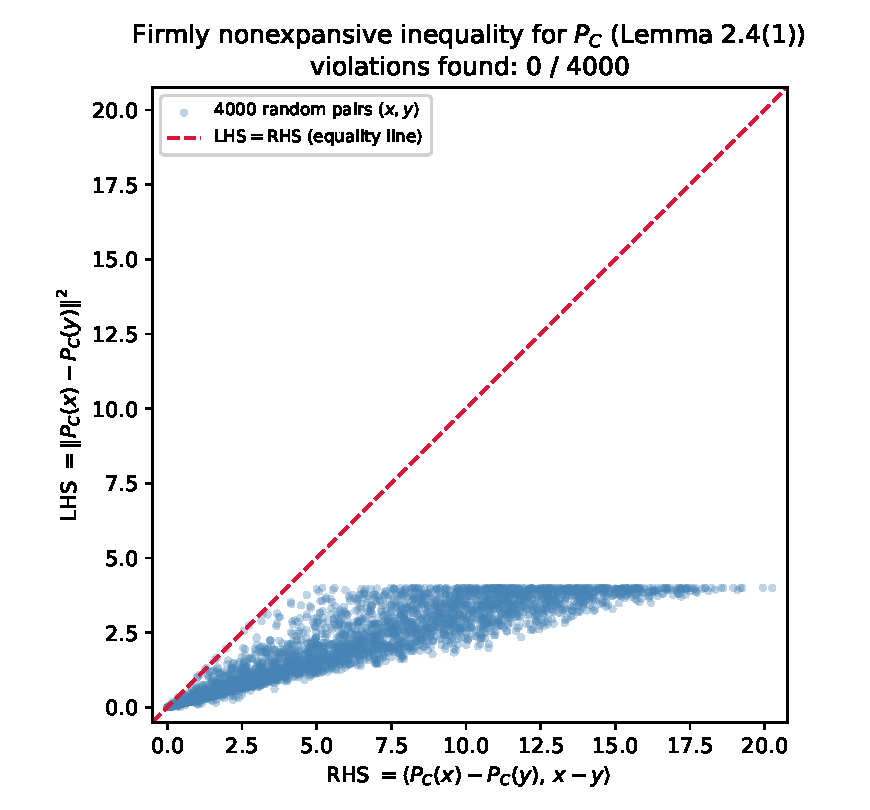
\includegraphics[height=5.6cm]{fig_firmly_nonexpansive}

  \small Every one of $4000$ random pairs $(x,y) \in \R^2 \times \R^2$
  satisfies $\|P_C(x)-P_C(y)\|^2 \le \langle P_C(x)-P_C(y), x-y\rangle$: all
  points fall on or below the equality line.
\end{frame}

%% ══════════════════════════════════════════════════════════════════════════
\section{Chapter Summary}
%% ══════════════════════════════════════════════════════════════════════════

\begin{frame}[allowframebreaks]{Chapter Summary: The Vocabulary Hierarchy}

  \begin{block}{Operator Classes, From Strongest to Weakest}
    \centering
    \begin{tabular}{ll}
      \toprule
      \textbf{Class} & \textbf{Key inequality / relation} \\
      \midrule
      Contractive & $\|Tx-Ty\|\le L\|x-y\|$, $L<1$ \\
      Firmly nonexpansive & $\|Tx-Ty\|^2 \le \langle Tx-Ty,x-y\rangle$ \\
      $\tfrac12$-averaged & special case of averaged, $\alpha=\tfrac12$ \\
      $\alpha$-averaged & $T=\alpha S+(1-\alpha)\Id$, $S$ nonexpansive \\
      Nonexpansive & $\|Tx-Ty\|\le \|x-y\|$ \\
      Quasi-nonexpansive & nonexpansive inequality, $y\in\Fix(T)$ only \\
      $k$-demicontractive & $\|Tx-y\|^2\le\|x-y\|^2+k\|Tx-x\|^2$ \\
      Pseudocontractive & $\|Tx-Ty\|^2\le\|x-y\|^2+\|(\Id-T)x-(\Id-T)y\|^2$ \\
      \bottomrule
    \end{tabular}
    \medskip

    Each class in this list contains all classes above it (e.g.\ every
    firmly nonexpansive map is $\tfrac12$-averaged, every averaged map is
    nonexpansive, every nonexpansive map with a fixed point is
    quasi-nonexpansive). $P_C$ sits near the top: it is firmly nonexpansive,
    hence $\tfrac12$-averaged, hence nonexpansive, hence (having fixed points)
    quasi-nonexpansive.
  \end{block}

  \framebreak

  \begin{block}{Convex-Analysis Vocabulary, Side by Side}
    \centering
    \begin{tabular}{ll}
      \toprule
      \textbf{Object} & \textbf{Role} \\
      \midrule
      Monotone operator $A$ & multivariate ``increasing function'' \\
      Maximally monotone $A$ & monotone, and cannot be enlarged \\
      Resolvent $J_{\gamma A}$ & $(\Id+\gamma A)^{-1}$, always firmly nonexpansive \\
      $\beta$-cocoercive $B$ & quantified monotone + Lipschitz \\
      $f \in \Gamma_0(\mathcal{H})$ & proper, convex, lower semi-continuous \\
      $\partial f$ & subdifferential; maximally monotone if $f\in\Gamma_0(\mathcal H)$ \\
      $\iota_C$, $N_C=\partial \iota_C$ & indicator function, normal cone \\
      $\operatorname{prox}_{\gamma f}$ & $J_{\gamma \partial f}$, firmly nonexpansive \\
      $\operatorname{prox}_{\iota_C}$ & equals $P_C$ exactly \\
      \bottomrule
    \end{tabular}
  \end{block}

  \begin{alertblock}{What Comes Next}
    Chapter 3 puts this vocabulary to work: the Krasnosel'ski\u{i}--Mann
    iteration $x_{n+1} = (1-\alpha_n)x_n + \alpha_n T(x_n)$ is precisely an
    averaging step applied to a nonexpansive (or more general) operator $T$,
    and its convergence proof will invoke Lemma~2.4 through 2.9, the
    demiclosedness principle, and the identity (2.4) introduced in this
    chapter -- all without re-deriving them.
  \end{alertblock}

\end{frame}

\end{document}
